\documentclass[10pt,a4paper]{article}
\usepackage[top=3cm,bottom=4cm,left=3.5cm,right=3.5cm]{geometry}
\usepackage{amsmath,amsthm,amsfonts,amssymb,amscd}
\usepackage{fancyhdr,color,comment,graphicx,environ,float,mathtools,mathrsfs,bbm,listings}
\newcommand{\norm}[1]{\left\lVert#1\right\rVert}

% Custom headers
\pagestyle{fancy}
\lhead{ECON - 8050}
\chead{}
\rhead{Tate Mason}
\lfoot{}
\cfoot{\thepage}

\begin{document}

\title{TakeHomeMidterm}
\author{Tate Mason}
\date{}
\maketitle

\section*{Life cycle model}
Consider the problem of a retired person who decumulates a given amount
of wealth $W$. He solves the following problem:

\begin{align*}
    \sum_{t=1}^{T} \beta^t u(c_t) \rightarrow \max_{c,k}
\end{align*}

s.t.\\
total resources of the household:
\begin{align*}
    res_t &= k_t(1 + r) + y_t - x_t\\
    k_1 &= W
\end{align*}

Here $k_t$ is savings, $y_t$ is pension income, and $x_t$ is medical expense shock.
There is a means-tested support program that guarantees each household
consumption at the level $c_{min}$ if his resources are too low. If $res_t > c_{min}$,
then $c_t = res_t - k_{t+1}$, $k_{t+1} \geq 0$. Else, $c_t = c_{min}$ and $k_{t+1} = 0$.

Solve the model using backward induction. Assume CRRA utility function with risk aversion $\sigma$: $u(c_t) = \frac{c_t^{1-\sigma}}{1-\sigma}$. Set $\beta = 0.95$, $r = 0.04$, $\sigma = 3$, $T = 40$, $c_{min} = 0.1$. For income, set $y_t = 1$ for all $t$. For initial wealth set $W = 10$.
Assume $x_t$ can take two values with probability 0.8 and 0.2. Download the
file containing the values for $x_t$ from the course website (xpts40.in). Discretize $k$ using 100 gridpoints, so that $k(1) = 0$ and $k(100) = 100$. Make sure
the grid is more dense around 0. When looking for optimal $k_{t+1}$ do NOT
restrict it to lie on the grid. Make sure you enforce the constraint $k_{t+1} \geq 0$.
(When looking for a maximum you can use Matlab command fminbnd.) To
find value function outside the grid of $k$ use linear interpolation. (When
doing linear interpolation command findnearest can be useful.)

\begin{enumerate}
    \item Solve the model and plot resulting policy functions for $k_{t+1}$ and value
function for ages 10 and 30 fixing $x_t$ at the 1st and 2nd grid.
Organize your graphs as follows: $2 \times 2$ matrix. Left column - savings,
right column - value function. Top row - for age 10, bottom row - age 30.
Each graph should have 2 lines (clearly labeled): fixing $x_t$ at the 1st and
2nd grid (command subplot in Matlab can be useful).

    \item Simulate $\{x_t\}$ for $t = 1 : 40$. Plot savings over the lifecycle using your
policy function.

    \item Increase $c_{min}$ to 0.5 and resolve the model. Plot savings over the life
cycle.

    \item Go back to $c_{min}$ equal to 0.1. Remove medical shock (set $x_t = 0$).
Resolve the model and plot savings over the lifecycle.

    \item Go back to the initial parametrization with medical shock and increase
$\beta$ to 0.99. Resolve the model and plot savings over the lifecycle.

    \item Combine saving profiles from questions 2-5 on the same graph and
compare. Make sure to clearly label each line. Provide economic intuition.
\end{enumerate}

\section*{Solutions}
\subsection*{Part 1}

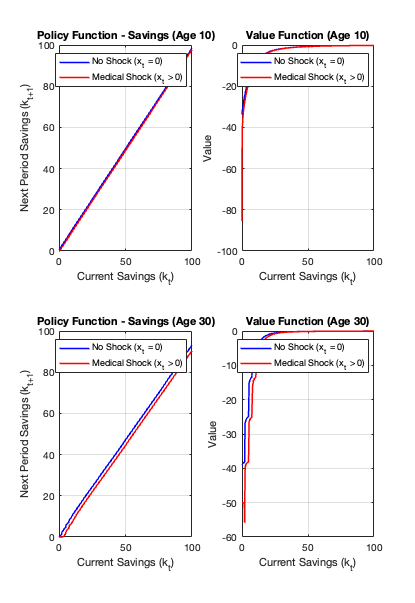
\includegraphics[scale=0.5]{solve_grid.png}

\subsection*{Part 2}

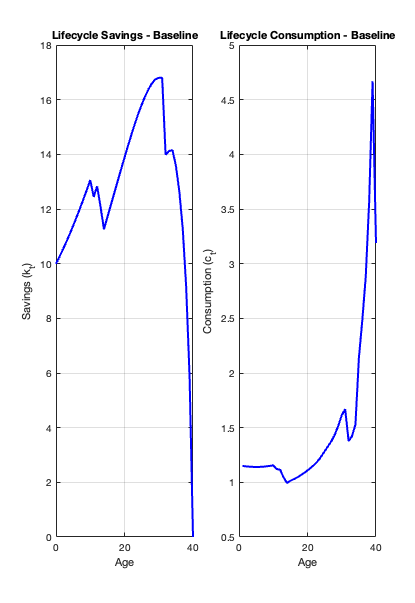
\includegraphics[scale=0.5]{baseline_lifecycle.png}

\subsection*{Part 3}

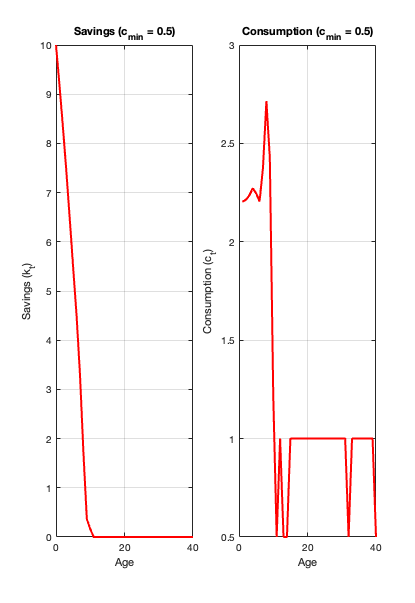
\includegraphics[scale=0.5]{higher_cmin_lifecycle.png}

\subsection*{Part 4}

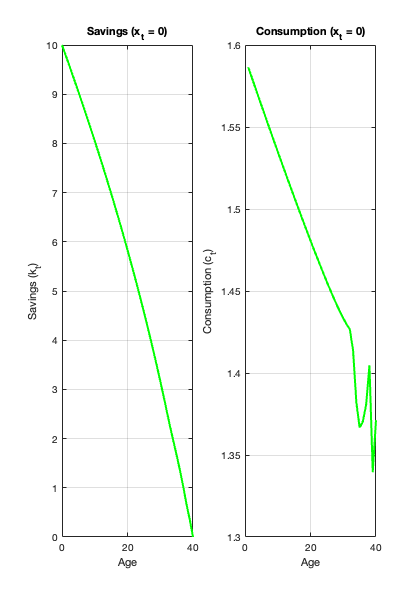
\includegraphics[scale=0.5]{no_shock_lifecycle.png}

\subsection*{Part 5}

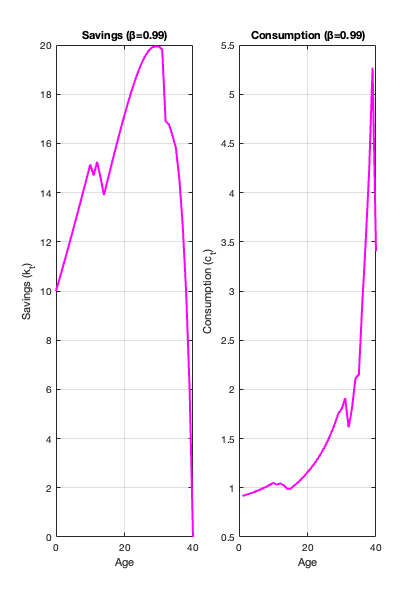
\includegraphics[scale=0.5]{high_beta_lifecycle.png}

\subsection*{Part 6}


As can be seen in the graph above, raising minimum consumption leads to less precautionary saving over the lifetime. As the floor is higher, there is less incentive to hold wealth, instead, agents will consume to meet their needs. In the case of getting rid of the medical shock, there is now incentive to save earlier due to the lack of uncertainty, and a much more linear curve for both savings and consumption. Now, when we raise the discounting rate, we can see an emphasized curve of the one from part 2. This makes sense as, with a higher level of patience (for lack of a better term), they will save more throughout, leading to a steeper decline as period $t=T$ approaches. 


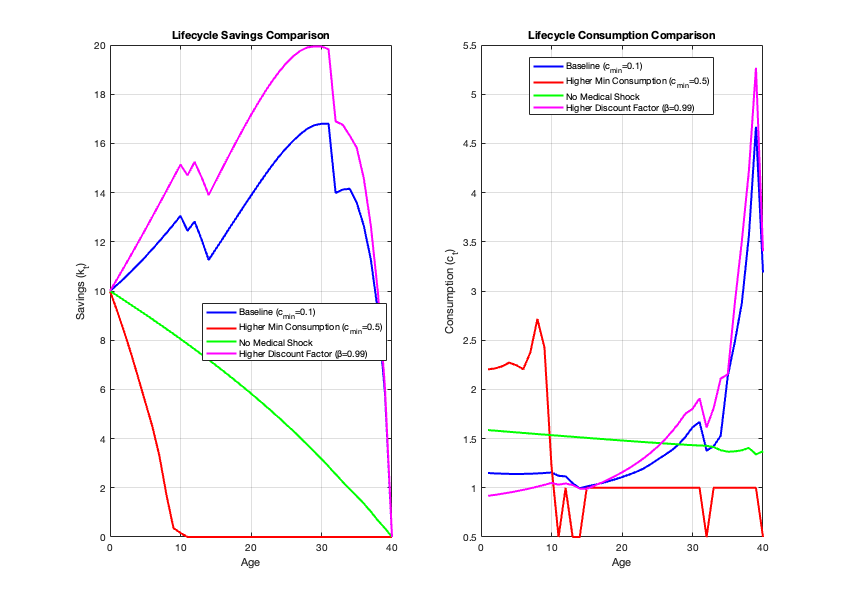
\includegraphics[scale=0.5]{lifecycle_comparison.png}
\begin{lstlisting}
%%%%%%%%%%%%%%%%%%%%%%%%%%%%%%%%%%%%%%%%%
%% Tate Mason - David.Mason2@uga.edu   %%
%% Midterm Exam - Take Home Section    %%
%% Due on Mar 17, 2025                 %%
%%%%%%%%%%%%%%%%%%%%%%%%%%%%%%%%%%%%%%%%%

clear;
clc;
close all;

%% Definition of Parameters %%

r = 0.04; % Interest rate
beta = 0.95; % Discount rate
sigma = 3; % Risk aversion
T = 40; % Time
cmin = 0.1; % Original minimum consumption level
y = 1; % Income from pension - constant 
W = 10; % Initial wealth
n = 100; % Number of points in kgrid

%% Definition of kgrid %%

kgrid = linspace(0,100^0.5, n).^2; % Creates a denser distribution of points near 0 and goes to 100

%% Definition of xgrid %%
x_data = load('xpts40.txt'); % Loads provided file

xgrid = [zeros(1,40); x_data(:,2)']; % Creates matrix which in the first row has no medical shock and in the second has transposed shocks
pX = [0.8;0.2]; % Definition of given probability of shock

%% Definition of CRRA Utility %%

u = @(c) (c.^(1-sigma))/(1-sigma);

%% Initialization of Value and Policy Functions %%

V = zeros(n,2,T); % Vt - n grid points, 2 shock values, and T periods of time
k_opt = zeros(n,2,T); % Optimal savings

%% Starting at t = T %%

for ik = 1:n % loop over kgrid
  for ix = 1:2 % loop over xgrid in cases of no shock and shock
    kt = kgrid(ik); % Current savings
    xt = xgrid(ix,T); % Current medical expense 
    
    totres = kt*(1+r) + y - xt; % Total resources
    if totres <= cmin;
      c = cmin;
      k_next = 0; % Final period --> no saving
    else
      c = totres;
      k_next = 0; % Final period --> no saving
    end
    V(ik, ix, T) = u(c); % Value function with found values
    k_opt(ik, ix, T) = k_next; % Optimal savings (0 in this case)
  end
end

%% Now Move Recursively %%

for t = (T-1):-1:1 % Starting at period T-1 and moving backwards through time
  for ik = 1:n
    for ix = 1:2
      kt = kgrid(ik);
      xt = xgrid(ix,t);
      totres = kt*(1+r) + y - xt;
      if totres <= cmin
        c = cmin;
        k_next = 0;
        V(ik,ix,t) = u(c);
      else
        obj = @(kp) -obj_func(kp,totres,beta,pX,kgrid,V(:,:,t+1),u); % Definition of function which is to be maximized
        [k_next, Eval] = fminbnd(obj,0,totres); % Find optimal savings for kt+1
        V(ik,ix,t) = -Eval; % Computation of value function, making sure to take negative of Eval as instructed
      end
      k_opt(ik,ix,t) = k_next; 
    end
  end
end

%% Plotting for Ages 10/30 %%

figure('Position', [100, 100, 1000, 800]); 

% t = 10
subplot(2,2,1);
plot(kgrid, k_opt(:,1,10), 'b', 'LineWidth',1.5); 
hold on;
plot(kgrid, k_opt(:,2,10), 'r', 'LineWidth',1.5); 
title('Policy Function - Savings (Age 10)');
xlabel('Current Savings (k_t)');
ylabel('Next Period Savings (k_{t+1})');
legend('No Shock (x_t = 0)', 'Medical Shock (x_t > 0)');
grid on;

subplot(2,2,2);
plot(kgrid, V(:,1,10), 'b', 'LineWidth', 1.5); 
hold on;
plot(kgrid, V(:,2,10), 'r', 'LineWidth', 1.5); 
title('Value Function (Age 10)');
xlabel('Current Savings (k_t)');
ylabel('Value');
legend('No Shock (x_t = 0)', 'Medical Shock (x_t > 0)');
grid on;

% t = 30
subplot(2,2,3);
plot(kgrid, k_opt(:,1,30), 'b', 'LineWidth', 1.5); 
hold on;
plot(kgrid, k_opt(:,2,30), 'r', 'LineWidth',1.5); 
title('Policy Function - Savings (Age 30)');
xlabel('Current Savings (k_t)');
ylabel('Next Period Savings (k_{t+1})');
legend('No Shock (x_t = 0)', 'Medical Shock (x_t > 0)');
grid on;

subplot(2,2,4);
plot(kgrid, V(:,1,30), 'b', 'LineWidth', 1.5); 
hold on;
plot(kgrid, V(:,2,30), 'r', 'LineWidth', 1.5);
title('Value Function (Age 30)');
xlabel('Current Savings (k_t)');
ylabel('Value');
legend('No Shock (x_t = 0)', 'Medical Shock (x_t > 0)');
grid on;


%% Simulation for baseline %%
rng(17); % Random seed set for reproducibility
simx = zeros(T,1);
draws = rand(T,1);

for t = 1:T
  if draws(t) <= pX(1)
    simx(t) = xgrid(1,t);
  else
    simx(t) = xgrid(2,t);
  end
end

ksim_baseline = zeros(T+1,1);
ksim_baseline(1) = W; % Initial wealth

% Also track consumption
csim_baseline = zeros(T,1);

for t = 1:T
  [~,idx_k] = min(abs(kgrid - ksim_baseline(t)));

  if simx(t) == xgrid(1,t)
    idx_x = 1;
  else
    idx_x = 2;
  end
  
  % Calculate total resources for consumption calculation
  totres = ksim_baseline(t)*(1+r) + y - simx(t);
  
  if abs(kgrid(idx_k)-ksim_baseline(t)) < 1e-6
    ksim_baseline(t+1) = k_opt(idx_k, idx_x, t);
  else
    if ksim_baseline(t) < kgrid(1)
      ksim_baseline(t+1) = k_opt(1, idx_x, t);  
    elseif ksim_baseline(t) > kgrid(end) 
      ksim_baseline(t+1) = k_opt(end, idx_x, t);  
    else 
      jlo = find(kgrid <= ksim_baseline(t), 1, 'last');
      jlo2 = jlo + 1;
      w = (ksim_baseline(t)-kgrid(jlo))/(kgrid(jlo2)-kgrid(jlo));
      ksim_baseline(t+1) = (1-w)*k_opt(jlo, idx_x, t) + w*k_opt(jlo2, idx_x, t); 
    end
  end
  
  % Calculate consumption as total resources minus next period savings
  if totres <= cmin
    csim_baseline(t) = cmin;
  else
    csim_baseline(t) = totres - ksim_baseline(t+1);
  end
end

% Plot baseline savings and consumption
figure('Position', [100, 100, 1000, 400]);

subplot(1,2,1);
plot(0:T, ksim_baseline, 'b-', 'LineWidth', 2);
title('Lifecycle Savings - Baseline');
xlabel('Age');
ylabel('Savings (k_t)');
grid on;

subplot(1,2,2);
plot(1:T, csim_baseline, 'b-', 'LineWidth', 2);
title('Lifecycle Consumption - Baseline');
xlabel('Age');
ylabel('Consumption (c_t)');
grid on;

saveas(gcf, 'baseline_lifecycle.png');

%% PART 3: Higher Minimum Consumption (cmin = 0.5) %%

% Preserve original cmin
cmin_og = cmin;

% Set higher cmin
cmin = 0.5;

% Initialize higher cmin value and policy functions
V_high_cmin = zeros(n,2,T);
k_opt_high_cmin = zeros(n,2,T);

% Starting at t = T for higher cmin
for ik = 1:n
  for ix = 1:2
    kt = kgrid(ik);
    xt = xgrid(ix,T);
    
    totres = kt*(1+r) + y - xt;
    if totres <= cmin
      c = cmin;
      k_next = 0;
    else
      c = totres;
      k_next = 0;
    end
    V_high_cmin(ik, ix, T) = u(c);
    k_opt_high_cmin(ik, ix, T) = k_next;
  end
end

% Move recursively for higher cmin
for t = (T-1):-1:1
  for ik = 1:n
    for ix = 1:2
      kt = kgrid(ik);
      xt = xgrid(ix,t);
      totres = kt*(1+r) + y - xt;
      if totres <= cmin
        c = cmin;
        k_next = 0;
        V_high_cmin(ik,ix,t) = u(c);
      else
        obj = @(kp) -obj_func(kp,totres,beta,pX,kgrid,V_high_cmin(:,:,t+1),u);
        [k_next,Eval] = fminbnd(obj,0,totres);
        V_high_cmin(ik,ix,t) = -Eval;
      end
      k_opt_high_cmin(ik,ix,t) = k_next;
    end
  end
end

% Simulation for higher cmin (using same shock sequence)
ksim_high_cmin = zeros(T+1,1);
ksim_high_cmin(1) = W;
csim_high_cmin = zeros(T,1);

for t = 1:T
  [~,idx_k] = min(abs(kgrid - ksim_high_cmin(t)));

  if simx(t) == xgrid(1,t)
    idx_x = 1;
  else
    idx_x = 2;
  end
  
  % Calculate total resources for consumption calculation
  totres = ksim_high_cmin(t)*(1+r) + y - simx(t);
  
  if abs(kgrid(idx_k)-ksim_high_cmin(t)) < 1e-6
    ksim_high_cmin(t+1) = k_opt_high_cmin(idx_k, idx_x, t);
  else
    if ksim_high_cmin(t) < kgrid(1)
      ksim_high_cmin(t+1) = k_opt_high_cmin(1, idx_x, t);  
    elseif ksim_high_cmin(t) > kgrid(end) 
      ksim_high_cmin(t+1) = k_opt_high_cmin(end, idx_x, t);  
    else 
      jlo = find(kgrid <= ksim_high_cmin(t), 1, 'last');
      jlo2 = jlo + 1;
      w = (ksim_high_cmin(t)-kgrid(jlo))/(kgrid(jlo2)-kgrid(jlo));
      ksim_high_cmin(t+1) = (1-w)*k_opt_high_cmin(jlo, idx_x, t) + w*k_opt_high_cmin(jlo2, idx_x, t); 
    end
  end
  
  % Calculate consumption as total resources minus next period savings
  if totres <= cmin
    csim_high_cmin(t) = cmin;
  else
    csim_high_cmin(t) = totres - ksim_high_cmin(t+1);
  end
end

% Plot higher cmin savings and consumption
figure('Position', [100, 100, 1000, 400]);

subplot(1,2,1);
plot(0:T, ksim_high_cmin, 'r-', 'LineWidth', 2);
title('Savings (c_{min} = 0.5)');
xlabel('Age');
ylabel('Savings (k_t)');
grid on;

subplot(1,2,2);
plot(1:T, csim_high_cmin, 'r-', 'LineWidth', 2);
title('Consumption (c_{min} = 0.5)');
xlabel('Age');
ylabel('Consumption (c_t)');
grid on;

saveas(gcf, 'higher_cmin_lifecycle.png');

%% PART 4: No Medical Shock (cmin = 0.1, xt = 0) %%

% Reset to original cmin
cmin = cmin_og;

% Initialize no-shock value and policy functions
V_no_shock = zeros(n,T);
k_opt_no_shock = zeros(n,T);

% Starting at t = T for no shock
for ik = 1:n
  kt = kgrid(ik);
  xt = 0; % No medical expense
  
  totres = kt*(1+r) + y - xt;
  if totres <= cmin
    c = cmin;
    k_next = 0;
  else
    c = totres;
    k_next = 0;
  end
  V_no_shock(ik, T) = u(c);
  k_opt_no_shock(ik, T) = k_next;
end

% Move recursively for no shock
for t = (T-1):-1:1
  for ik = 1:n
    kt = kgrid(ik);
    xt = 0; % No medical expense
    totres = kt*(1+r) + y - xt;
    if totres <= cmin
      c = cmin;
      k_next = 0;
      V_no_shock(ik,t) = u(c);
    else
      % For no shock case, we use a simplified objective function
      obj = @(kp) -obj_func_no_shock(kp,totres,beta,kgrid,V_no_shock(:,t+1),u);
      [k_next,Eval] = fminbnd(obj,0,totres);
      V_no_shock(ik,t) = -Eval;
    end
    k_opt_no_shock(ik,t) = k_next;
  end
end

% Simulation for no shock case
ksim_no_shock = zeros(T+1,1);
ksim_no_shock(1) = W;
csim_no_shock = zeros(T,1);

for t = 1:T
  [~,idx_k] = min(abs(kgrid - ksim_no_shock(t)));
  
  % No medical shock, so total resources calculation is simpler
  totres = ksim_no_shock(t)*(1+r) + y;
  
  if abs(kgrid(idx_k)-ksim_no_shock(t)) < 1e-6
    ksim_no_shock(t+1) = k_opt_no_shock(idx_k, t);
  else
    if ksim_no_shock(t) < kgrid(1)
      ksim_no_shock(t+1) = k_opt_no_shock(1, t);  
    elseif ksim_no_shock(t) > kgrid(end) 
      ksim_no_shock(t+1) = k_opt_no_shock(end, t);  
    else 
      jlo = find(kgrid <= ksim_no_shock(t), 1, 'last');
      jlo2 = jlo + 1;
      w = (ksim_no_shock(t)-kgrid(jlo))/(kgrid(jlo2)-kgrid(jlo));
      ksim_no_shock(t+1) = (1-w)*k_opt_no_shock(jlo, t) + w*k_opt_no_shock(jlo2, t); 
    end
  end
  
  % Calculate consumption as total resources minus next period savings
  if totres <= cmin
    csim_no_shock(t) = cmin;
  else
    csim_no_shock(t) = totres - ksim_no_shock(t+1);
  end
end

% Plot no shock savings and consumption
figure('Position', [100, 100, 1000, 400]);

subplot(1,2,1);
plot(0:T, ksim_no_shock, 'g-', 'LineWidth', 2);
title('Savings (x_t = 0)');
xlabel('Age');
ylabel('Savings (k_t)');
grid on;

subplot(1,2,2);
plot(1:T, csim_no_shock, 'g-', 'LineWidth', 2);
title('Consumption (x_t = 0)');
xlabel('Age');
ylabel('Consumption (c_t)');
grid on;

saveas(gcf, 'no_shock_lifecycle.png');

%% PART 5: Higher Discount Factor (cmin = 0.1, beta = 0.99) %%

% Reset cmin to original and increase beta
cmin = cmin_og;
beta_high = 0.99;

% Initialize high-beta value and policy functions
V_high_beta = zeros(n,2,T);
k_opt_high_beta = zeros(n,2,T);

% Starting at t = T for high beta
for ik = 1:n
  for ix = 1:2
    kt = kgrid(ik);
    xt = xgrid(ix,T);
    
    totres = kt*(1+r) + y - xt;
    if totres <= cmin
      c = cmin;
      k_next = 0;
    else
      c = totres;
      k_next = 0;
    end
    V_high_beta(ik, ix, T) = u(c);
    k_opt_high_beta(ik, ix, T) = k_next;
  end
end

% Move recursively for high beta
for t = (T-1):-1:1
  for ik = 1:n
    for ix = 1:2
      kt = kgrid(ik);
      xt = xgrid(ix,t);
      totres = kt*(1+r) + y - xt;
      if totres <= cmin
        c = cmin;
        k_next = 0;
        V_high_beta(ik,ix,t) = u(c);
      else
        obj = @(kp) -obj_func(kp,totres,beta_high,pX,kgrid,V_high_beta(:,:,t+1),u);
        [k_next,Eval] = fminbnd(obj,0,totres);
        V_high_beta(ik,ix,t) = -Eval;
      end
      k_opt_high_beta(ik,ix,t) = k_next;
    end
  end
end

% Simulation for high beta (using same shock sequence)
ksim_high_beta = zeros(T+1,1);
ksim_high_beta(1) = W;
csim_high_beta = zeros(T,1);

for t = 1:T
  [~,idx_k] = min(abs(kgrid - ksim_high_beta(t)));

  if simx(t) == xgrid(1,t)
    idx_x = 1;
  else
    idx_x = 2;
  end
  
  % Calculate total resources for consumption calculation
  totres = ksim_high_beta(t)*(1+r) + y - simx(t);
  
  if abs(kgrid(idx_k)-ksim_high_beta(t)) < 1e-6
    ksim_high_beta(t+1) = k_opt_high_beta(idx_k, idx_x, t);
  else
    if ksim_high_beta(t) < kgrid(1)
      ksim_high_beta(t+1) = k_opt_high_beta(1, idx_x, t);  
    elseif ksim_high_beta(t) > kgrid(end) 
      ksim_high_beta(t+1) = k_opt_high_beta(end, idx_x, t);  
    else 
      jlo = find(kgrid <= ksim_high_beta(t), 1, 'last');
      jlo2 = jlo + 1;
      w = (ksim_high_beta(t)-kgrid(jlo))/(kgrid(jlo2)-kgrid(jlo));
      ksim_high_beta(t+1) = (1-w)*k_opt_high_beta(jlo, idx_x, t) + w*k_opt_high_beta(jlo2, idx_x, t); 
    end
  end
  
  % Calculate consumption as total resources minus next period savings
  if totres <= cmin
    csim_high_beta(t) = cmin;
  else
    csim_high_beta(t) = totres - ksim_high_beta(t+1);
  end
end

% Plot high beta savings and consumption
figure('Position', [100, 100, 1000, 400]);

subplot(1,2,1);
plot(0:T, ksim_high_beta, 'm-', 'LineWidth', 2);
title('Savings (β=0.99)');
xlabel('Age');
ylabel('Savings (k_t)');
grid on;

subplot(1,2,2);
plot(1:T, csim_high_beta, 'm-', 'LineWidth', 2);
title('Consumption (β=0.99)');
xlabel('Age');
ylabel('Consumption (c_t)');
grid on;

saveas(gcf, 'high_beta_lifecycle.png');

%% PART 6: Combine and Compare Saving and Consumption Profiles %%

% Combined Savings Plot
figure('Position', [100, 100, 1000, 400]);

subplot(1,2,1);
plot(0:T, ksim_baseline, 'b-', 'LineWidth', 2);
hold on;
plot(0:T, ksim_high_cmin, 'r-', 'LineWidth', 2);
plot(0:T, ksim_no_shock, 'g-', 'LineWidth', 2);
plot(0:T, ksim_high_beta, 'm-', 'LineWidth', 2);
title('Lifecycle Savings Comparison');
xlabel('Age');
ylabel('Savings (k_t)');
legend('Baseline (c_{min}=0.1)', 'Higher Min Consumption (c_{min}=0.5)', ...
       'No Medical Shock', 'Higher Discount Factor (β=0.99)', 'Location', 'best');
grid on;

subplot(1,2,2);
plot(1:T, csim_baseline, 'b-', 'LineWidth', 2);
hold on;
plot(1:T, csim_high_cmin, 'r-', 'LineWidth', 2);
plot(1:T, csim_no_shock, 'g-', 'LineWidth', 2);
plot(1:T, csim_high_beta, 'm-', 'LineWidth', 2);
title('Lifecycle Consumption Comparison');
xlabel('Age');
ylabel('Consumption (c_t)');
legend('Baseline (c_{min}=0.1)', 'Higher Min Consumption (c_{min}=0.5)', ...
       'No Medical Shock', 'Higher Discount Factor (β=0.99)', 'Location', 'best');
grid on;

saveas(gcf, 'lifecycle_comparison.png');

%% Helper Functions %%

function val = obj_func(kp, totres, beta, pX, kgrid, V_next, u)
  c = totres - kp;
  current_u = u(c);

  if kp <= kgrid(1)
    jlo = 1;
  elseif kp >= kgrid(end)
    jlo = length(kgrid)-1;
  else
    jlo = find(kgrid <= kp, 1, 'last');
  end
  jlo2 = jlo+1; 
  w = (kp - kgrid(jlo))/(kgrid(jlo2)-kgrid(jlo));
  Eval = 0;

  for ixp = 1:2
    v_next = (1-w)*V_next(jlo,ixp) + w*V_next(jlo2,ixp);     
    Eval = Eval + pX(ixp)*v_next;
  end
  val = current_u + beta*Eval;
end

function val = obj_func_no_shock(kp, totres, beta, kgrid, V_next, u)
  c = totres - kp;
  current_u = u(c);

  if kp <= kgrid(1)
    jlo = 1;
  elseif kp >= kgrid(end)
    jlo = length(kgrid)-1;
  else
    jlo = find(kgrid <= kp, 1, 'last');
  end
  jlo2 = jlo+1; 
  w = (kp - kgrid(jlo))/(kgrid(jlo2)-kgrid(jlo));
  
  % For no shock case, we only have one value in V_next per grid point
  v_next = (1-w)*V_next(jlo) + w*V_next(jlo2);
  
  val = current_u + beta*v_next;
end
\end{lstlisting}
\end{document}
